\subsection{Question 1}
\subsubsection{Part A}

\newpage
\subsubsection{Part B}

\lstinputlisting[caption=Matlab Commands,showstringspaces=false,language=Matlab]{../lu_sym.m}

\subsubsection{Part C}
The complexity of Gauss elimination is is \(O(\frac{m^{3}}{3})\).
Regular gauss elimination works on an entire matrix ({\em i.e.,} touching all elements of the matrix) during \(LU\) factorization.
However, for a symmetric matrix we have proven in part A that we only need to touch the upper triangular elements of a matrix.
This constitutes half of the matrix.
Therefore, the complexity of the symmetric \(LU\) factorization algorithm will be \(\frac{1}{2}\frac{m^{3}}{3}\) or simply \(O(\frac{m^{3}}{6})\).

\newpage
\subsubsection{Part D}

\newpage
\subsection{Question 2}
\subsubsection{Part A}

\newpage
\subsubsection{Part B}

\newpage
\subsubsection{Part C}

\newpage
\subsection{Question 3}
\subsubsection{Part A}

\newpage
\subsubsection{Part B}

\newpage
\subsubsection{Part C}

\newpage
\subsubsection{Part D}




%\lstinputlisting[caption=Matlab Commands,showstringspaces=false,language=Matlab]{../find_vectors.m}


%\begin{figure}[th]
%  \centering
%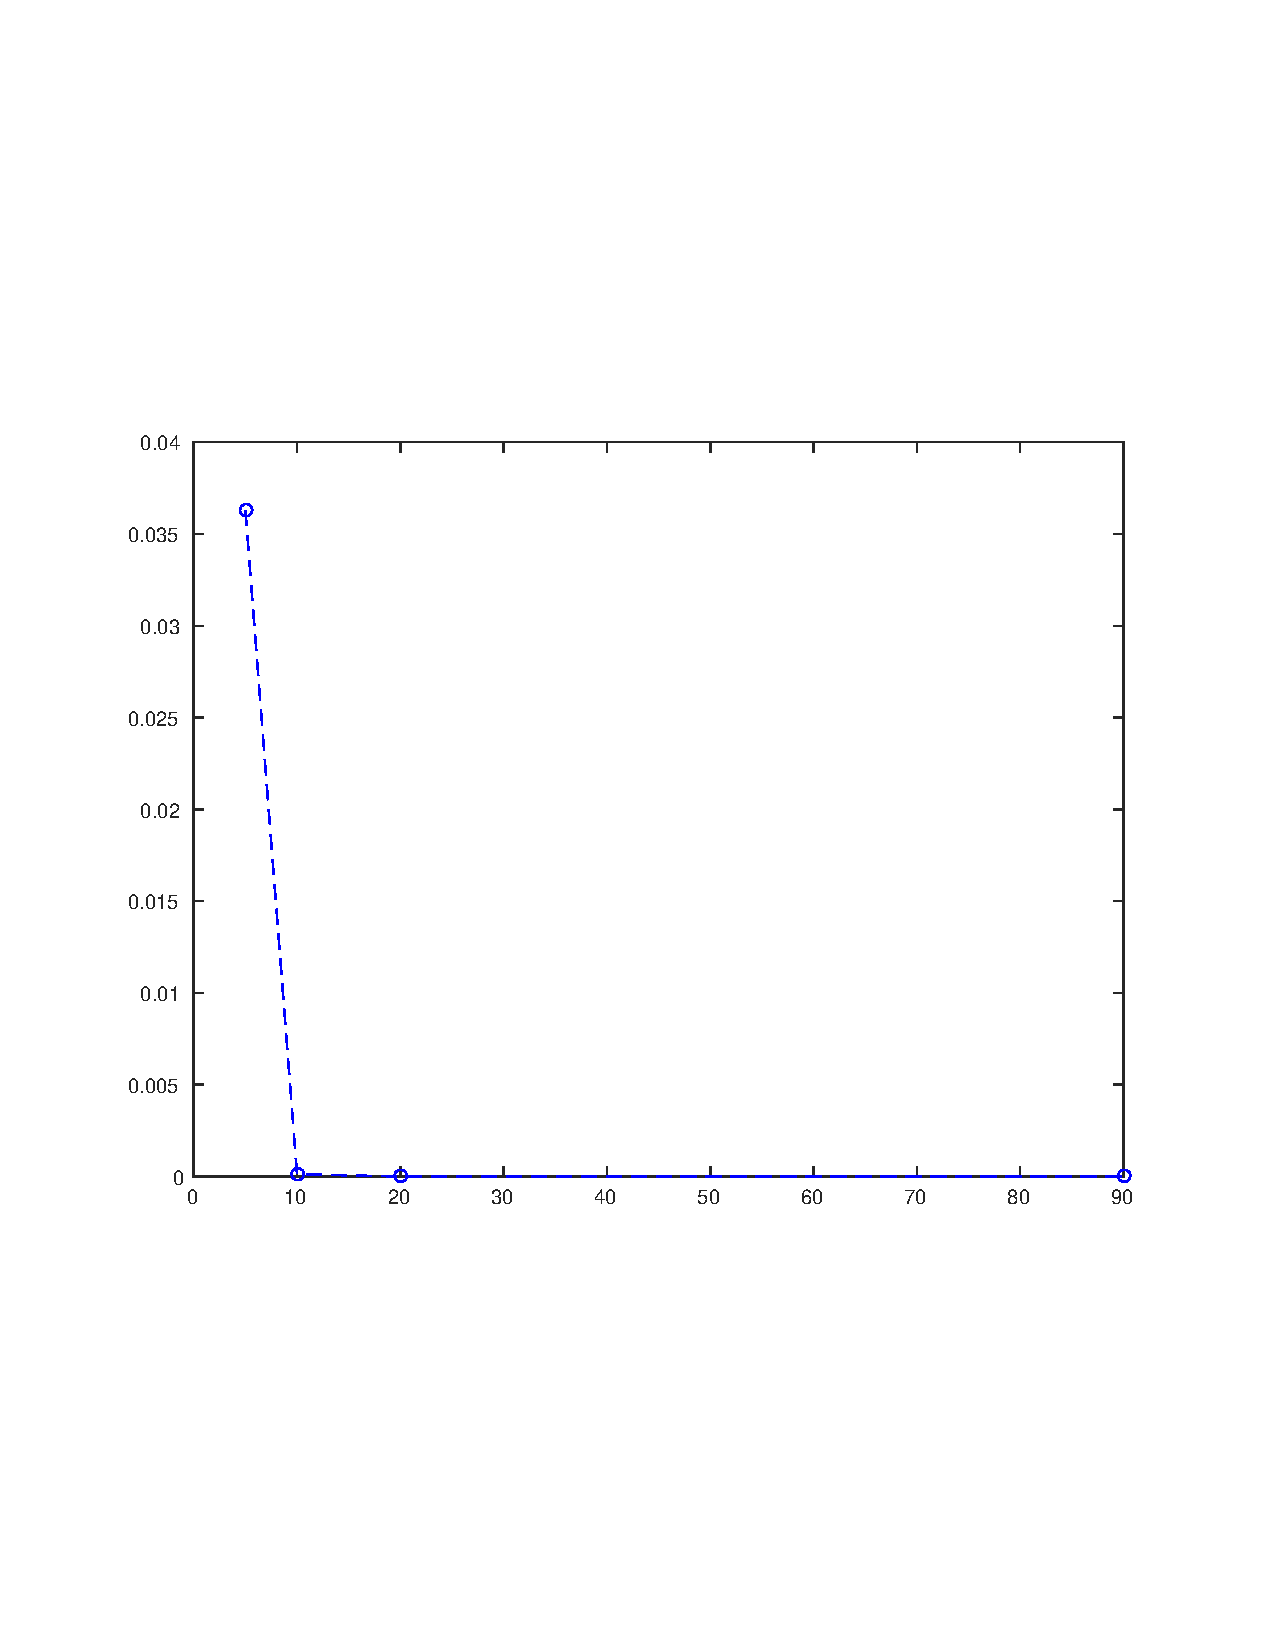
\includegraphics[trim=10mm 70mm 10mm 70mm, width=1.0\textwidth]{../q2_plots}
%\end{figure}
